\documentclass[11pt,a4paper]{article}

\usepackage[margin=0.7in]{geometry}
\usepackage{graphicx}
\usepackage{hyperref}
\usepackage{booktabs}
\usepackage{enumitem}
\usepackage{listings}
\usepackage{xcolor}
\usepackage{float}
\usepackage{longtable}
\usepackage{caption}
\usepackage{subcaption}

\hypersetup{
    colorlinks=true,
    linkcolor=blue,
    urlcolor=blue,
    citecolor=blue
}

\lstset{
    basicstyle=\ttfamily\small,
    breaklines=true,
    frame=single,
    backgroundcolor=\color{gray!10},
    columns=fullflexible
}

\title{%
    \textbf{ECSE 429 Software Validation} \\[0.5em]
    Part C: Non-Functional Testing of REST API \\[0.3em]
    Written Report
}
\author{
    Emile Labrunie (261097953) -- \texttt{emile.labrunie@mail.mcgill.ca} \\
    Ethan Wu (261117309) -- \texttt{ethan.wu2@mail.mcgill.ca} \\
    Kenny Duy Nguyen (261120429) -- \texttt{kenny.nguyen@mail.mcgill.ca} \\
    Yanzhe Zhang (261016377) -- \texttt{yanzhe.zhang@mail.mcgill.ca}
}
\date{Winter 2026}

\begin{document}

\maketitle
\tableofcontents
\newpage

%% ============================================================
\section{Introduction}
%% ============================================================

This report presents the non-functional testing performed on the REST API Todo List Manager application as Part~C of the ECSE~429 term project. Building on the functional validation conducted in Parts~A and~B, this phase focuses on two complementary aspects of software quality: \emph{performance testing} (dynamic analysis) and \emph{static analysis} of the application source code.

The performance testing component measures transaction time, CPU usage, and available free memory as the number of managed objects increases, providing insight into scalability and resource consumption. The static analysis component applies automated tooling to the Java codebase to identify code smells, potential bugs, security vulnerabilities, and areas of technical debt.

Together, these analyses inform concrete recommendations for improving the maintainability, reliability, and efficiency of the Todo Manager API.

%% ============================================================
\section{Summary of Deliverables}
%% ============================================================

The deliverables for Part~C are as follows:
\begin{itemize}
    \item \textbf{Performance test suite} -- A JavaScript program that creates, updates, and deletes objects via the REST API while measuring transaction time, CPU usage, and free memory at increasing object counts.
    \item \textbf{Performance charts} -- Graphs showing transaction time, CPU usage, and free memory versus number of objects for each entity type (todos, projects, categories).
    \item \textbf{Static analysis report} -- Results from running SpotBugs~4.7.3 on the compiled Java source code of the Todo Manager, including categorised findings and code change recommendations.
    \item \textbf{Performance test suite video} -- A recording of all performance tests running in our development environment.
    \item \textbf{This written report} (PDF, 5--10 pages), covering performance test implementation, findings, charts, performance risks and recommendations, static analysis implementation, findings, and code improvement recommendations.
\end{itemize}

%% ============================================================
\section{Implementation and Findings of Performance Test Suite}
%% ============================================================

\subsection{Implementation}

The dynamic analysis was implemented using a custom Node.js performance test suite. The suite is designed to incrementally stress the REST API by scaling the number of entities ($N$) and measuring the system's response across three core metrics: transaction latency, CPU utilization, and free memory.

The experimental setup and execution followed these parameters:
\begin{itemize}
    \item \textbf{Technology Stack:} The test script was written in JavaScript using Node.js. The \texttt{axios} library was used to execute the HTTP requests (POST, PUT, DELETE), and custom data generation scripts (\texttt{randomData.js}) populated the payloads.
    \item \textbf{Transaction Timing:} Latency was measured using the Node.js \texttt{perf\_hooks} module (\texttt{performance.now()}), providing high-resolution, sub-millisecond timing for each individual transaction.
    \item \textbf{System Metrics:} CPU percentage and free available memory were tracked natively using the Node.js \texttt{os} module. To ensure accuracy, the script calculated the CPU delta over a 500ms window running concurrently (via \texttt{Promise.all}) with the HTTP request batches.
    \item \textbf{Data Scaling:} The suite tested the API under logarithmically increasing loads, specifically seeding the database with $N \in \{1, 10, 50, 100, 500, 1000\}$ objects.
    \item \textbf{Server Lifecycle:} To isolate the variables, the Java JAR file (\texttt{runTodoManagerRestAPI-1.5.5.jar}) was started manually in a separate terminal process. Because the test script systematically deletes all created objects at the end of each iteration, the database state was reset naturally without requiring a hard server reboot between values of $N$.
\end{itemize}

\subsection{Findings}

The performance of the API was evaluated across all three primary entity types: Todos, Projects, and Categories. The following charts illustrate the transaction times, CPU utilization, and free memory degradation as $N$ scaled from 1 to 1000. 

\emph{Note: The $X$-axis representing the number of objects ($N$) is plotted on a logarithmic scale (Base 10) to accurately visualize the exponential scaling behavior.}

\subsubsection{Transaction Time Analysis}

\begin{figure}[H]
    \centering
    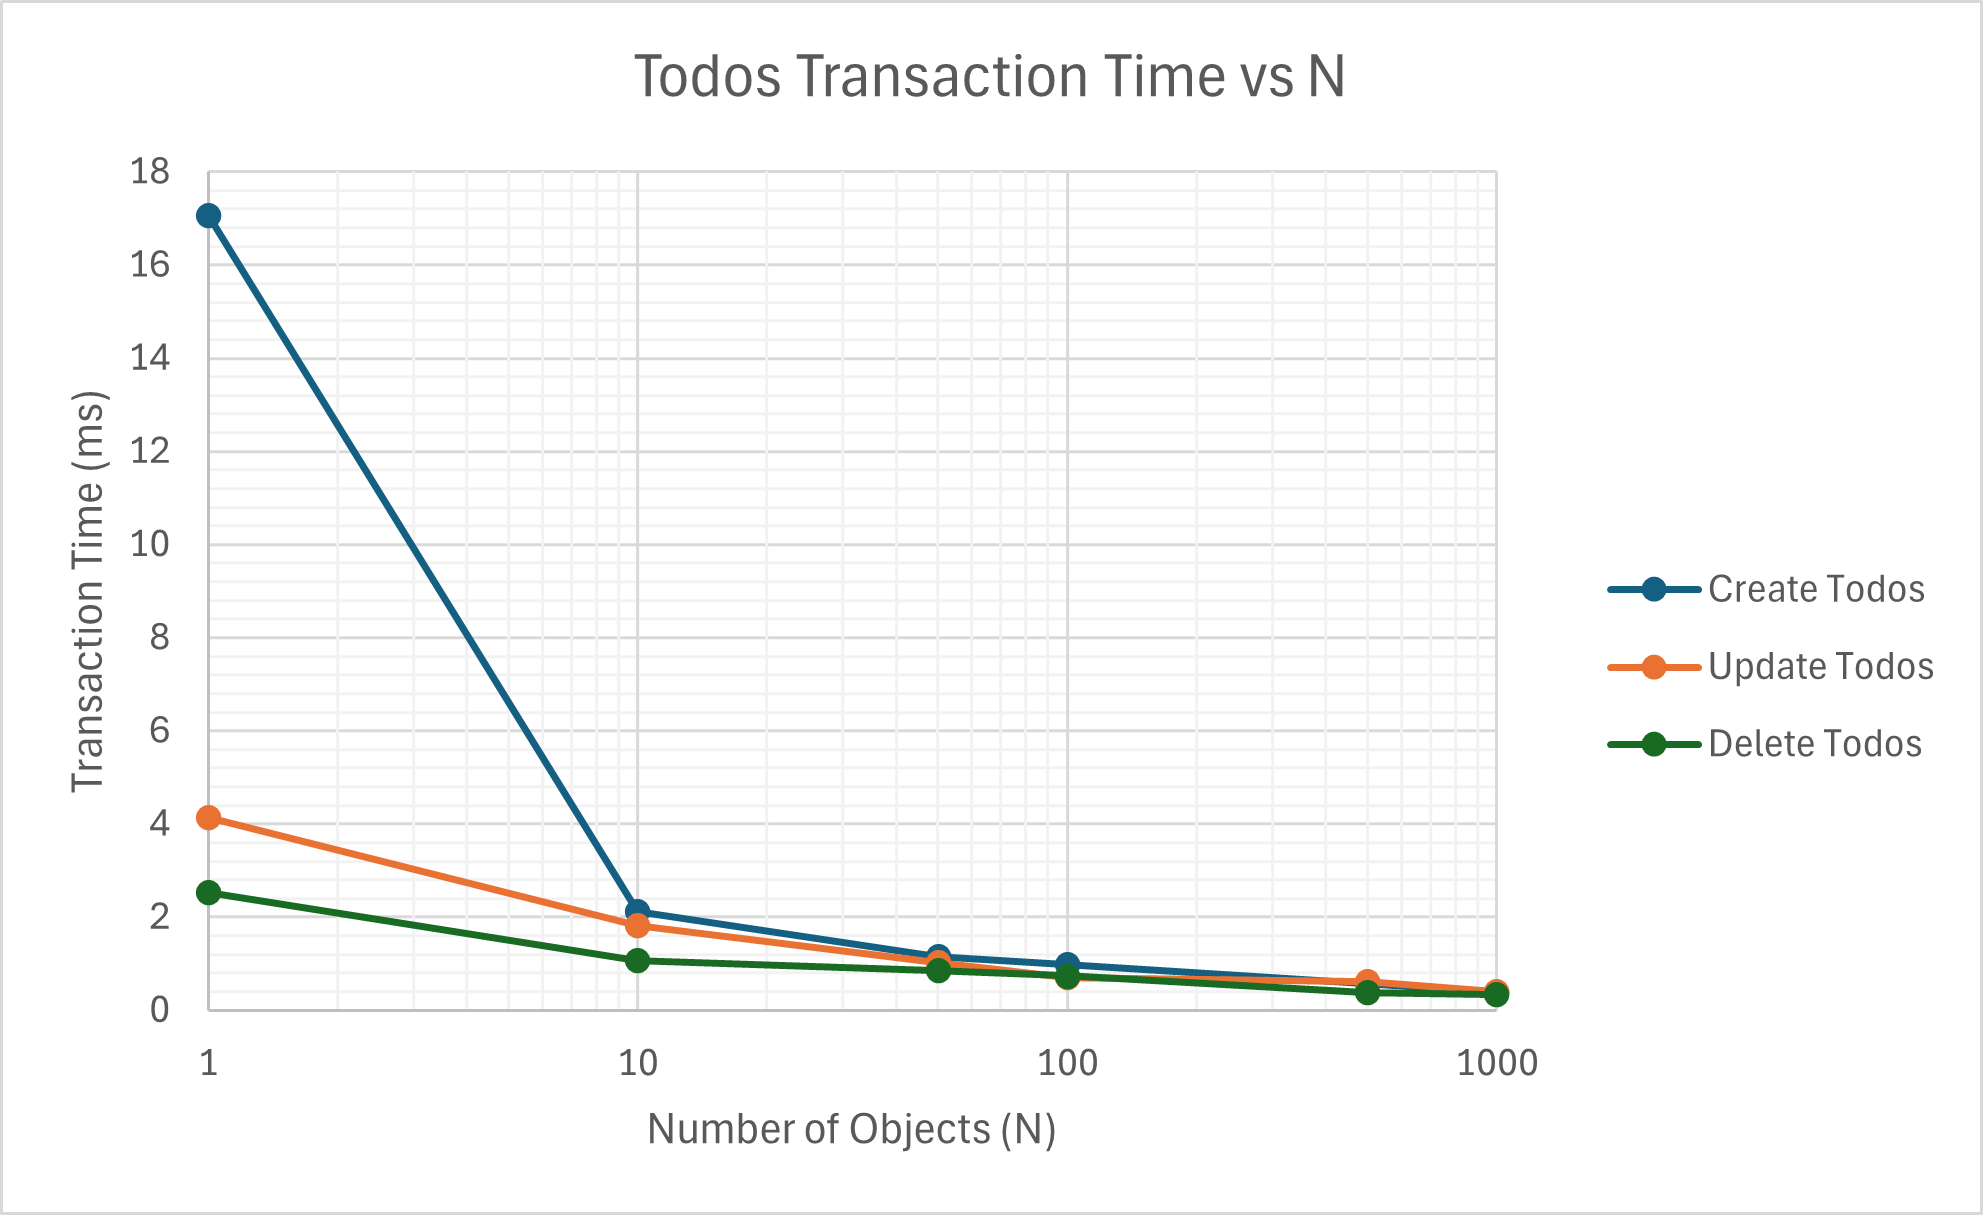
\includegraphics[width=0.8\textwidth]{figures/Todos_Time.png}
    \caption{Todo transaction time (ms) versus the number of objects ($N$).}
    \label{fig:todo-time}
\end{figure}

\begin{figure}[H]
    \centering
    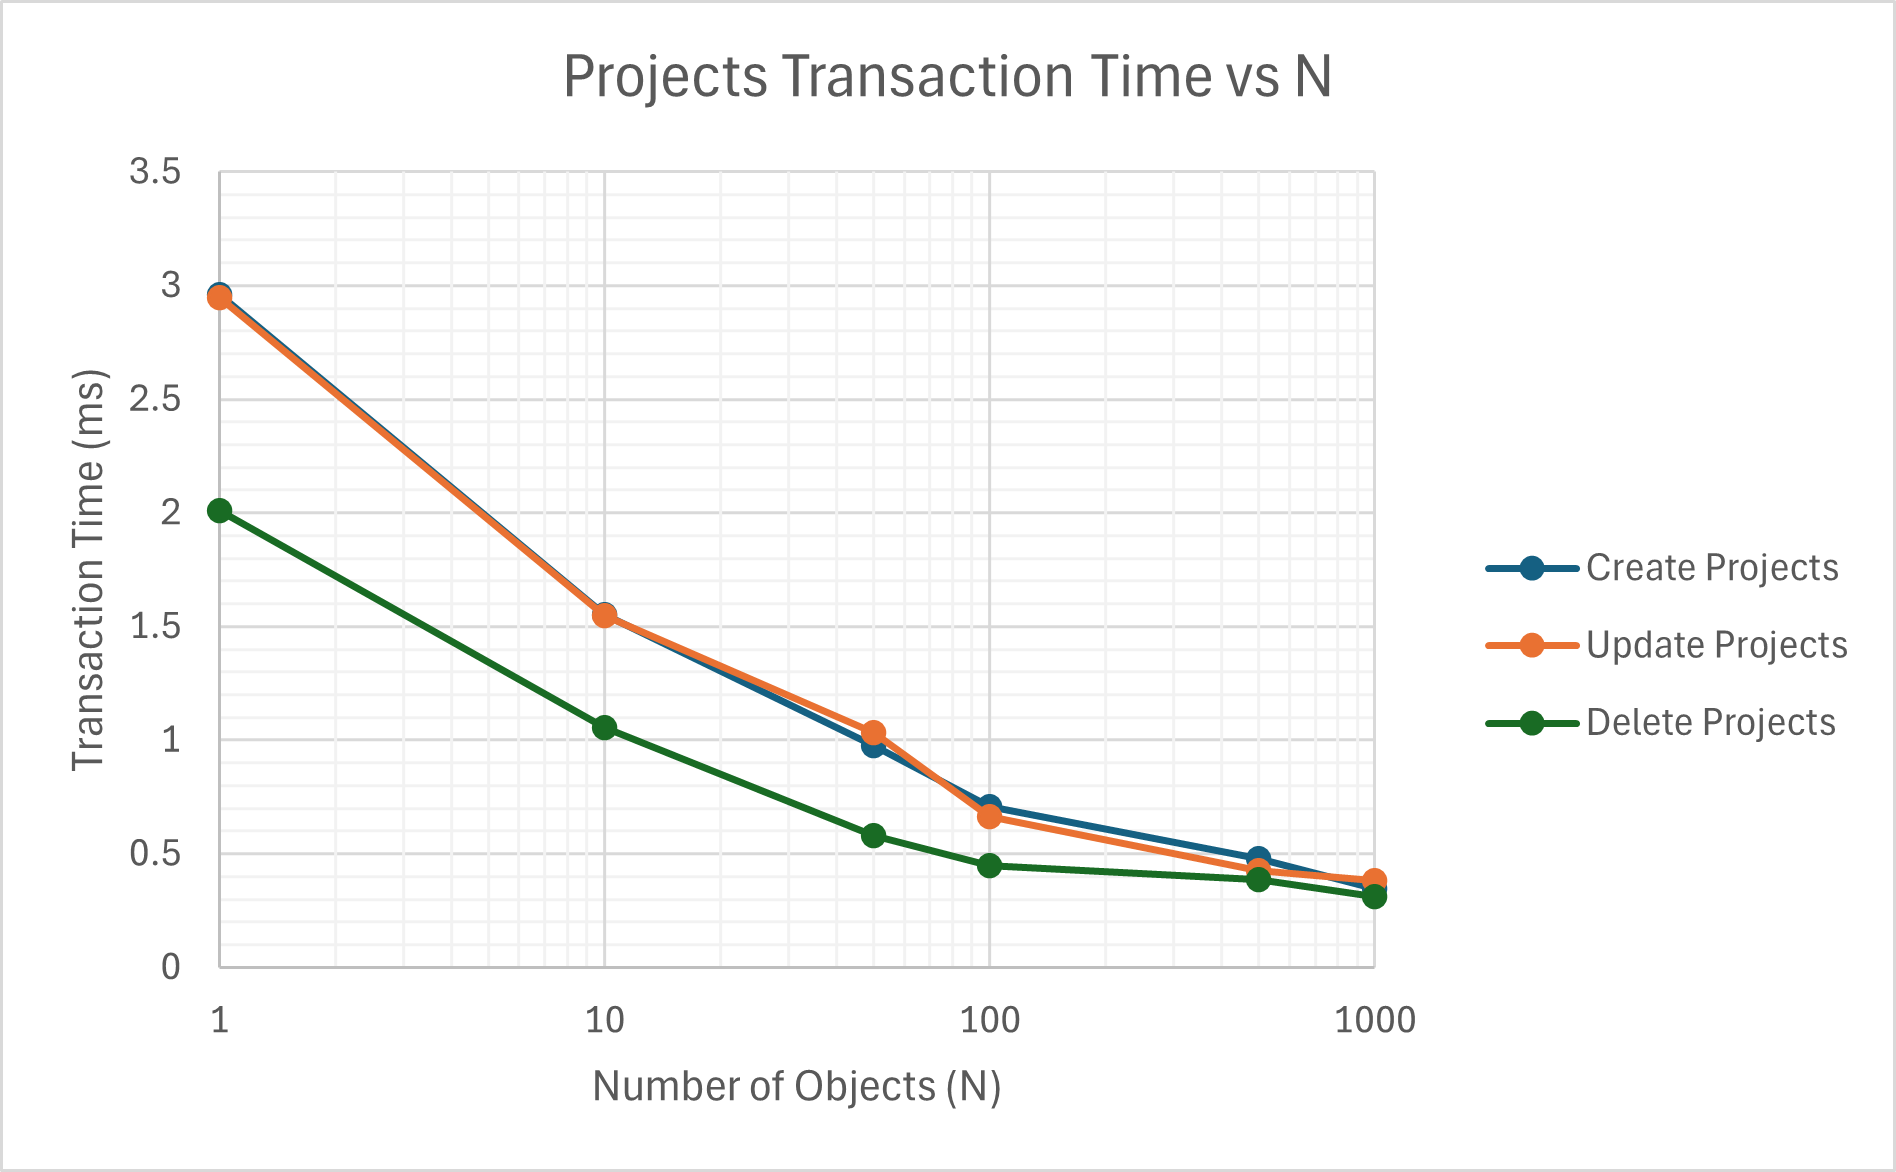
\includegraphics[width=0.8\textwidth]{figures/Projects_Time.png}
    \caption{Project transaction time (ms) vs.\ number of objects.}
    \label{fig:project-time}
\end{figure}

\begin{figure}[H]
    \centering
    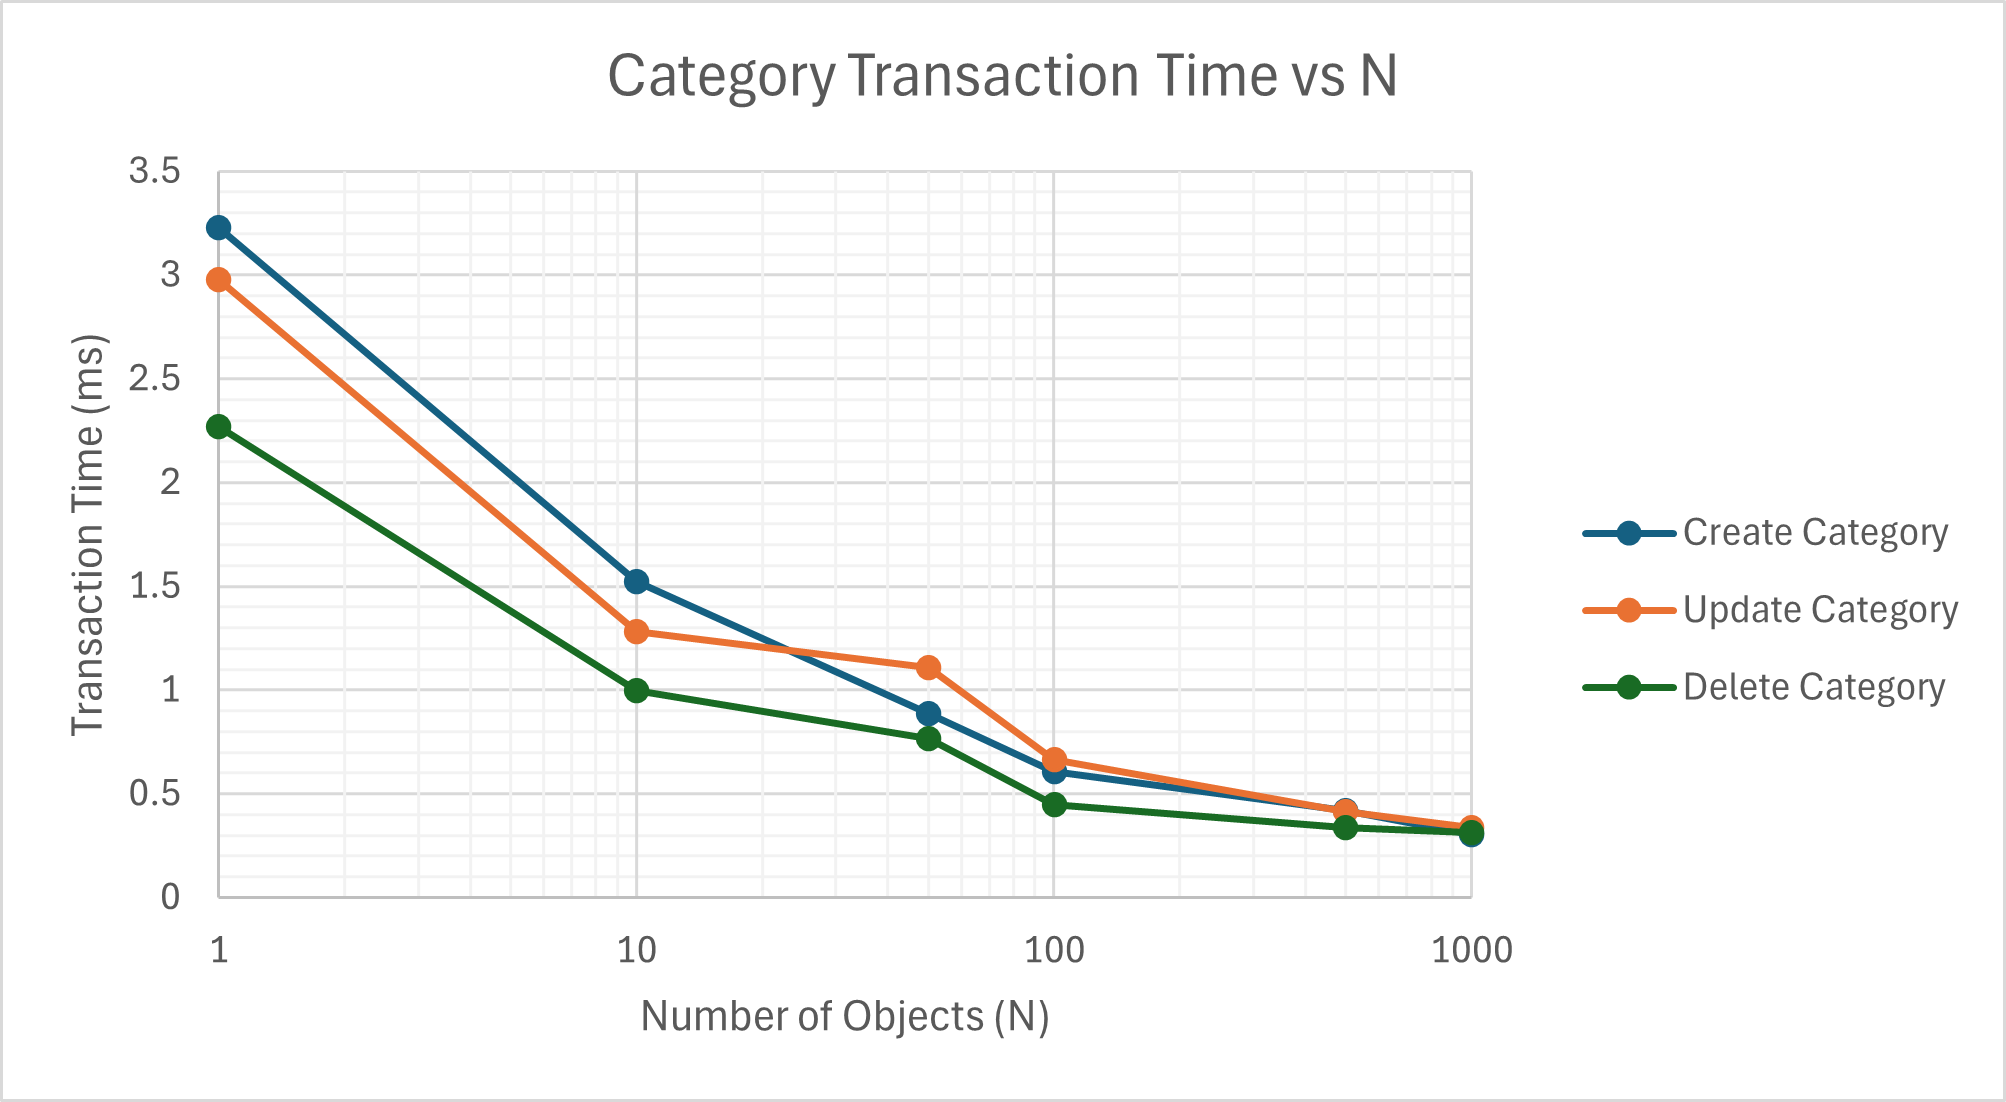
\includegraphics[width=0.8\textwidth]{figures/Category_Time.png}
    \caption{Category transaction time (ms) vs.\ number of objects.}
    \label{fig:category-time}
\end{figure}


\subsubsection{CPU Utilization Analysis}

\begin{figure}[H]
    \centering
    \includegraphics[width=0.8\textwidth]{figures/Todos_CPU_Percent.png}
    \caption{Todo CPU utilization (\%) vs.\ number of objects.}
    \label{fig:todo-cpu}
\end{figure}

\begin{figure}[H]
    \centering
    \includegraphics[width=0.8\textwidth]{figures/Projects_CPU_Percent.png}
    \caption{Project CPU utilization (\%) vs.\ number of objects.}
    \label{fig:project-cpu}
\end{figure}

\begin{figure}[H]
    \centering
    \includegraphics[width=0.8\textwidth]{figures/Category_CPU_Percent.png}
    \caption{Category CPU utilization (\%) vs.\ number of objects.}
    \label{fig:category-cpu}
\end{figure}


\subsubsection{Free Memory Degradation}

\begin{figure}[H]
    \centering
    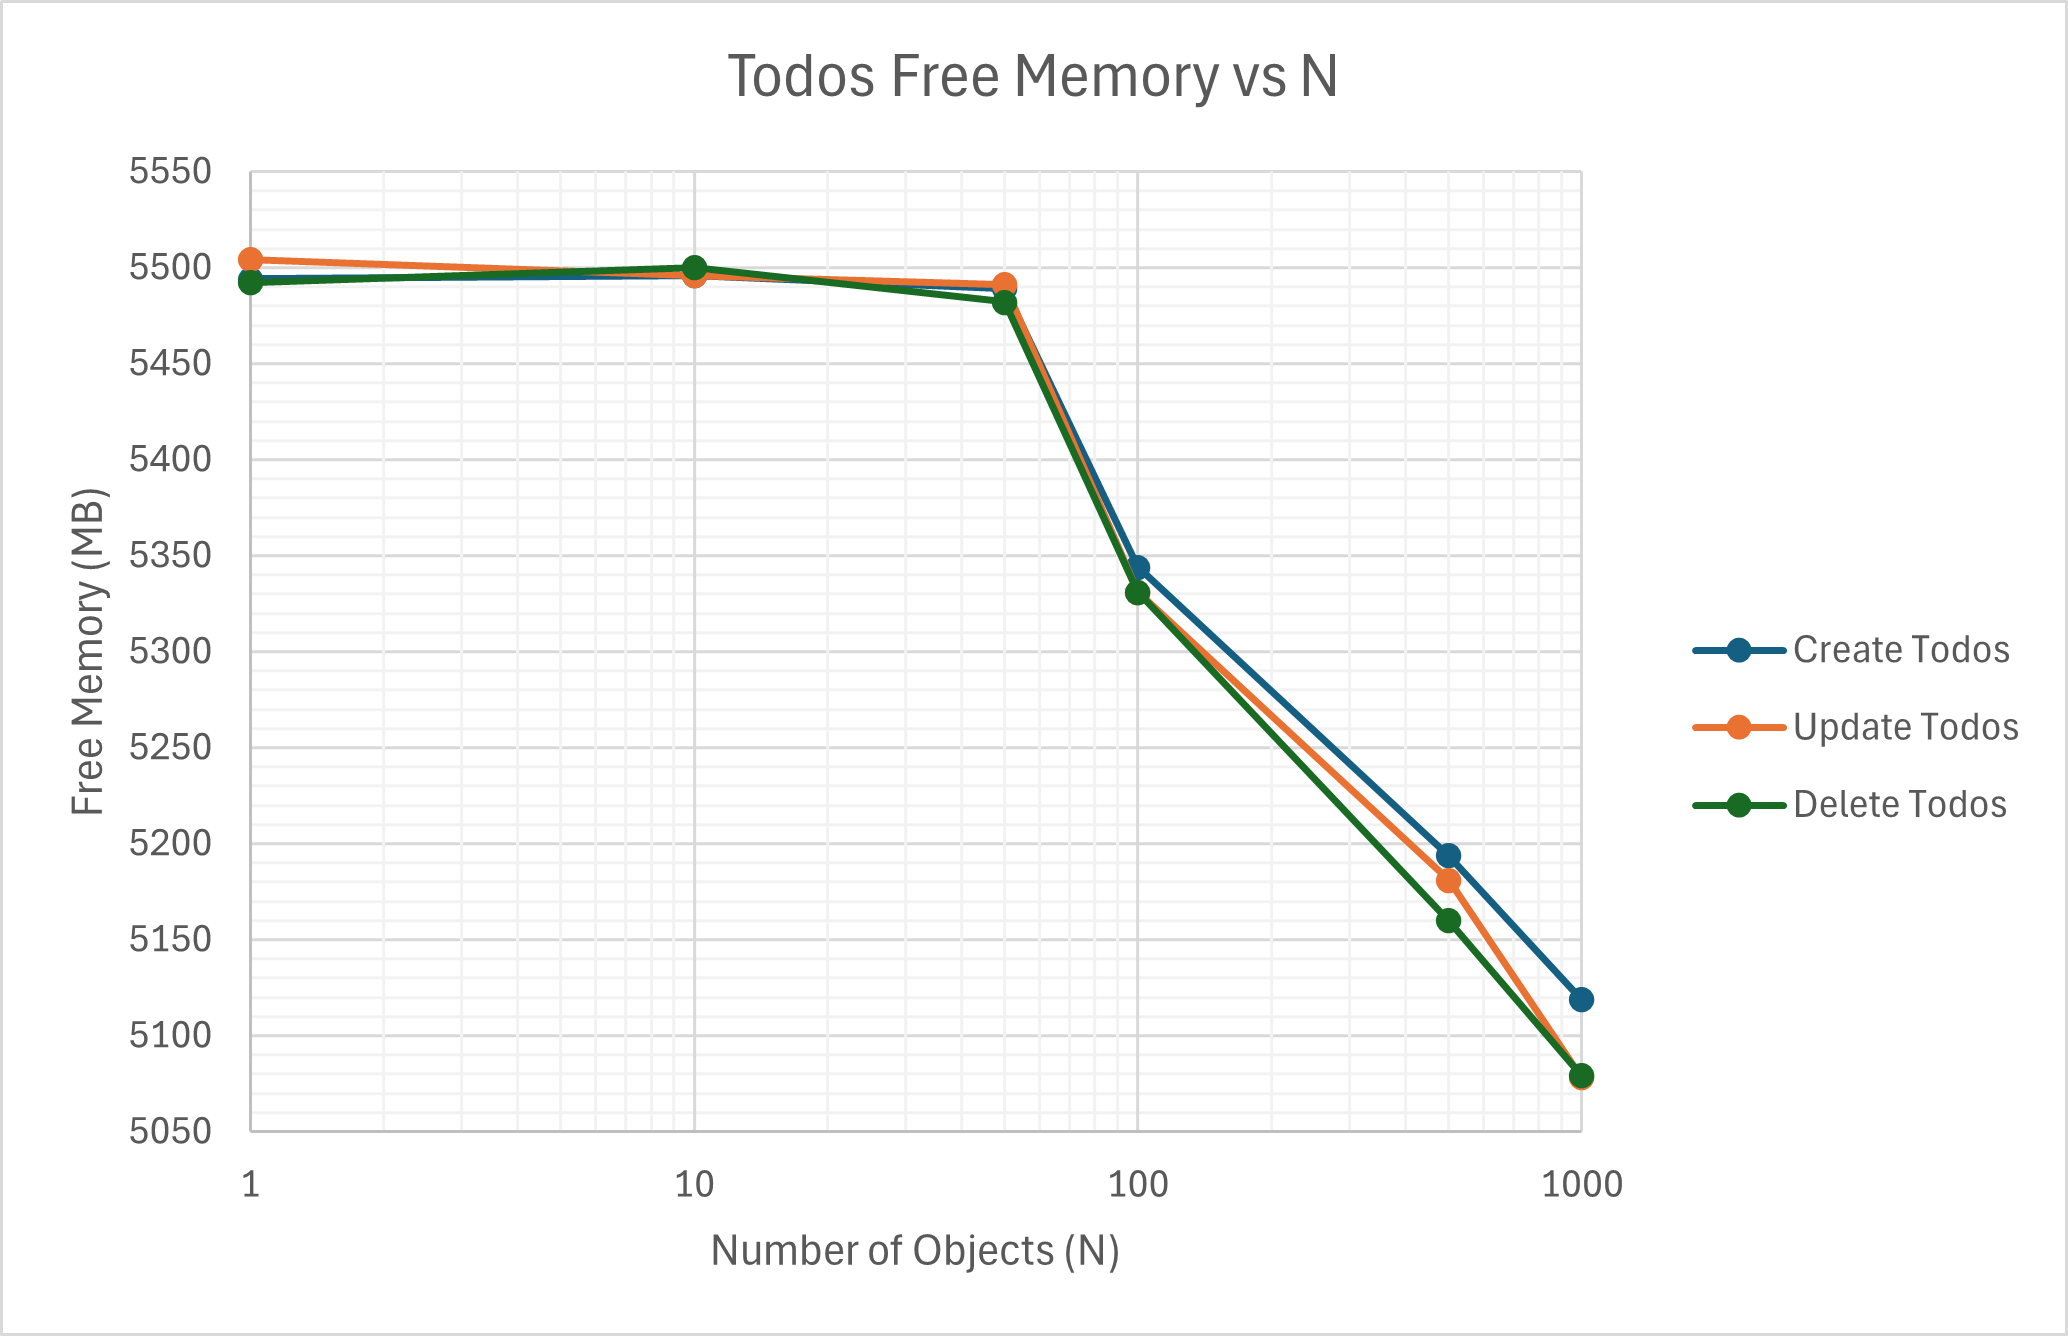
\includegraphics[width=0.8\textwidth]{figures/Todos_Free_Memory.png}
    \caption{Todo free memory (MB) vs.\ number of objects.}
    \label{fig:todo-memory}
\end{figure}

\begin{figure}[H]
    \centering
    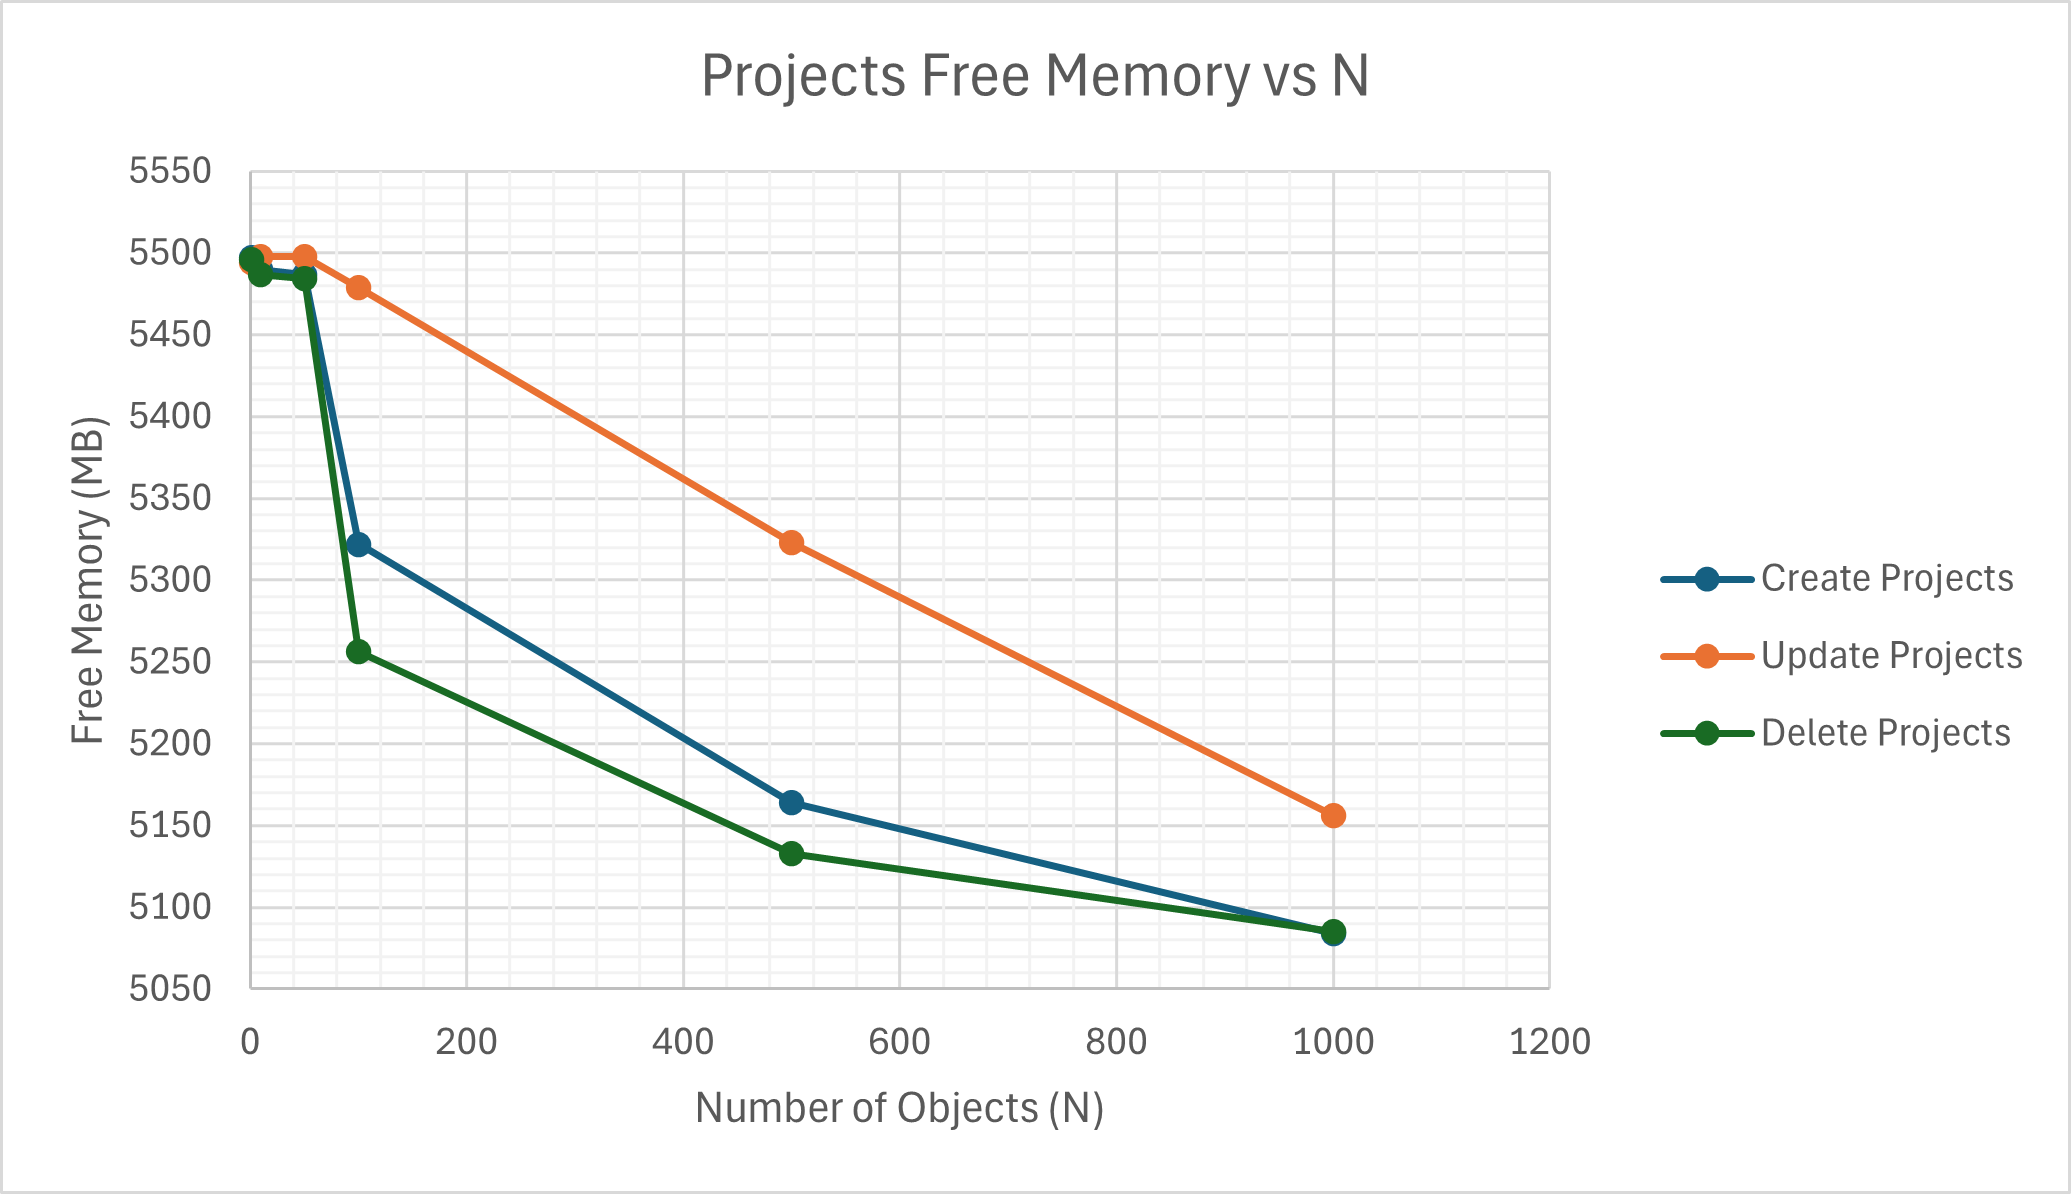
\includegraphics[width=0.8\textwidth]{figures/Projects_Free_Memory.png}
    \caption{Project free memory (MB) vs.\ number of objects.}
    \label{fig:project-memory}
\end{figure}

\begin{figure}[H]
    \centering
    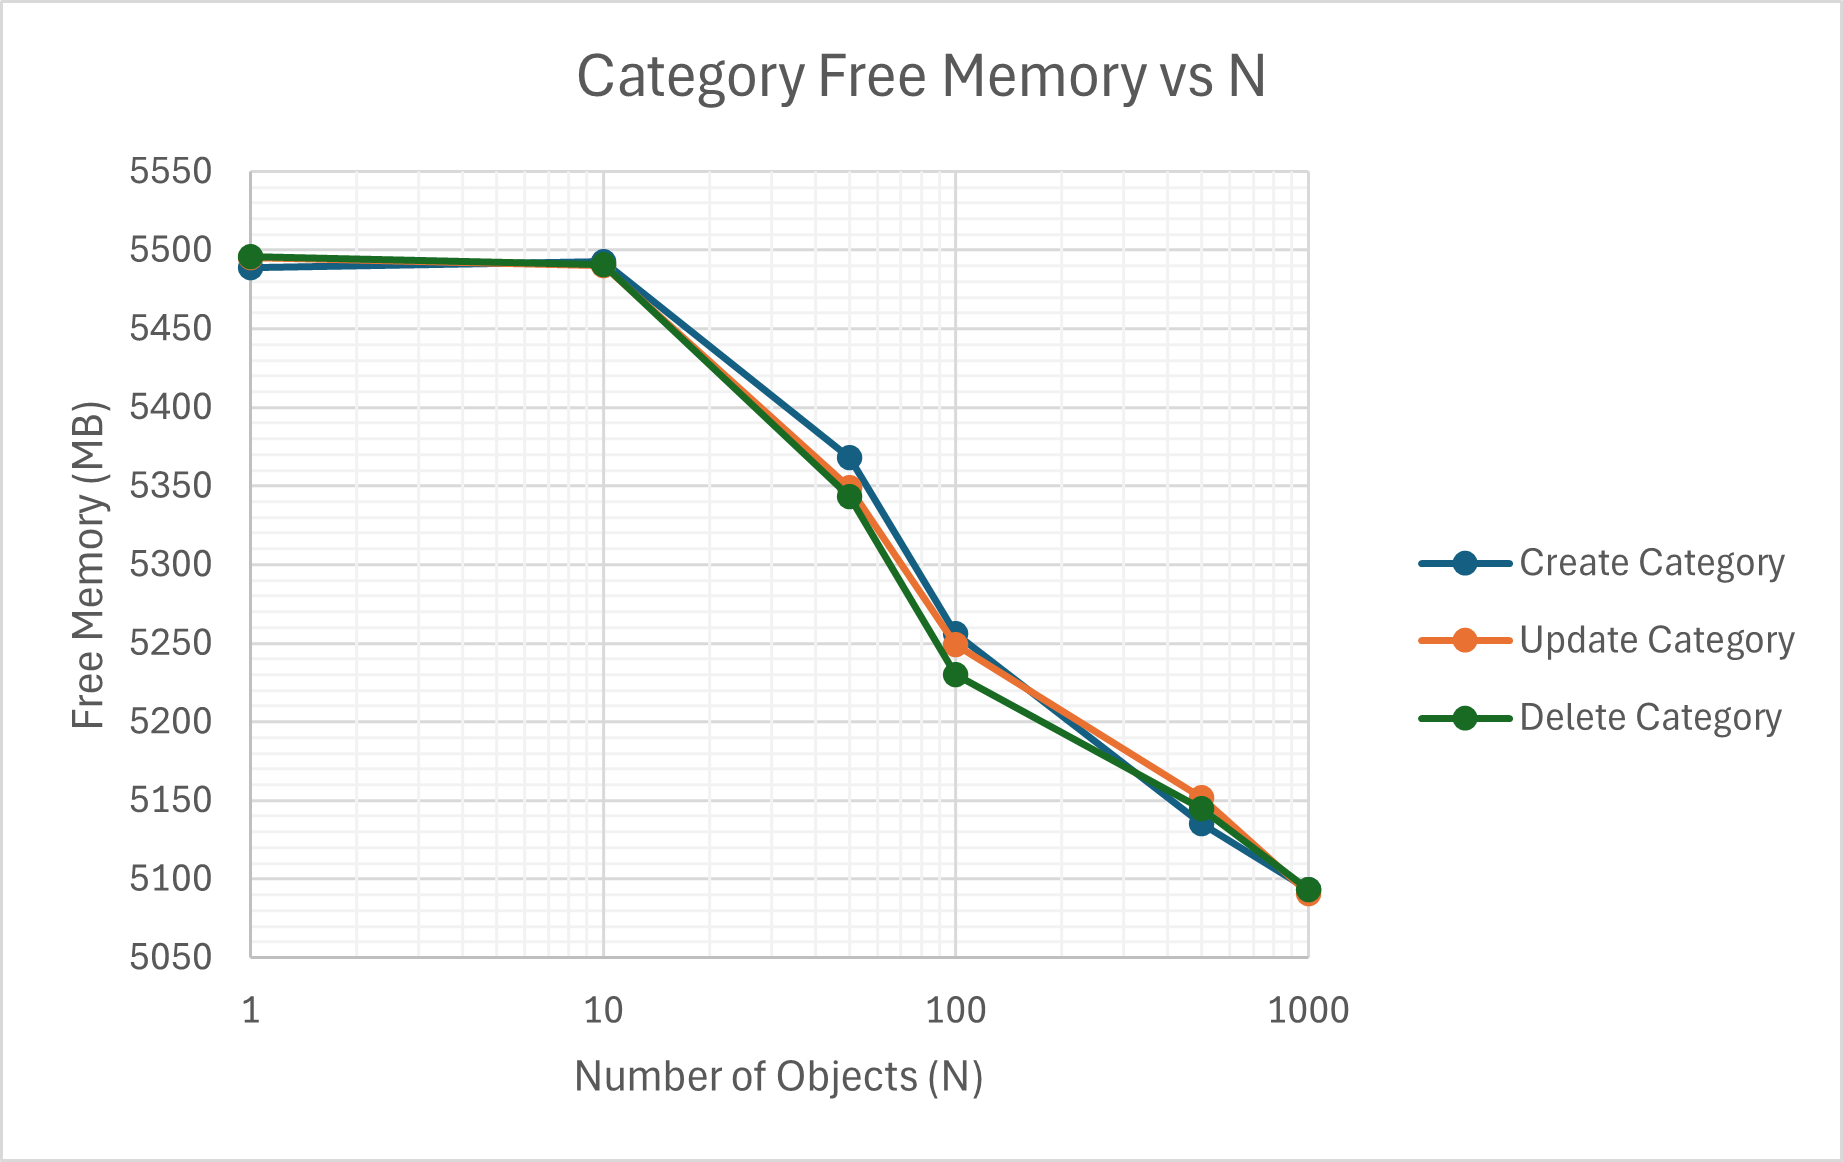
\includegraphics[width=0.8\textwidth]{figures/Category_Free_Memory.png}
    \caption{Category free memory (MB) vs.\ number of objects.}
    \label{fig:category-memory}
\end{figure}


\subsection{Performance Risks and Recommendations}

Analysis of the dynamic metrics reveals that while the API routes efficiently, it struggles significantly with resource management as the database scales. We observed the following key risks and propose corresponding recommendations:

\begin{itemize}
    \item \textbf{Risk: Severe Memory Bloat/Leak.} The most critical finding is the aggressive degradation of free memory. At $N=1$, the system reported 5494 MB of free memory. By $N=1000$, this dropped to 5078 MB. The system consumed over 400 MB of RAM to store 1,000 simple text objects (roughly 400 KB per object), which is disproportionately large for standard JSON payloads. If the application scales to 10,000+ objects, the Java heap will likely exhaust its limits, triggering an \texttt{OutOfMemoryError} and crashing the server.
    \item \textbf{Risk: Concurrency Bottlenecks (CPU Spikes).} While transaction times remained consistently low (sub-millisecond at $N=1000$), the CPU effort required to achieve those times scaled aggressively. CPU utilization spiked from $\sim$5\% at $N=10$ to peaking over 45\% at $N=500$ for single-threaded requests. In a production environment with concurrent users, the CPU would quickly bottleneck at 100\%, leading to locked threads and dropped requests.
    \item \textbf{The "JVM Warmup" Effect.} Transaction times showed a steep drop from $N=1$ ($\sim$17ms) to $N=1000$ ($\sim$0.3ms). This is a normal characteristic of the Java Virtual Machine (JVM) performing Just-In-Time compilation and class loading on the first request, and poses no risk.
\end{itemize}

\textbf{Recommendations:}
\begin{enumerate}
    \item \textbf{Heap Profiling:} Utilize a memory profiler (such as VisualVM) to analyze heap dumps during high-$N$ loads to identify which objects or data structures are responsible for the 400 MB memory consumption.
    \item \textbf{Audit Data Structures:} The combined memory bloat and CPU spikes suggest the internal "database" may be using inefficient data structures, such as performing deep copies of large \texttt{ArrayLists} or Maps on every transaction. Static analysis should be directed toward optimizing collection usage.
    \item \textbf{Garbage Collection Tuning:} Investigate unclosed streams or lingering object references (as supported by the static analysis findings) that may be preventing the JVM's Garbage Collector from reclaiming memory after HTTP requests conclude.
\end{enumerate}

%% ============================================================
\section{Static Analysis}
%% ============================================================

\subsection{Implementation}

Static analysis was performed on the compiled Java source code of the REST API Todo Manager, obtained from the \texttt{eviltester/thingifier} GitHub repository (\url{https://github.com/eviltester/thingifier}). The project was built using Maven (\texttt{mvn compile}) to produce the \texttt{.class} files required by the analysis tool.

We used \textbf{SpotBugs~4.7.3}, an open-source static analysis tool for Java bytecode that detects potential bugs, performance issues, bad coding practices, and security vulnerabilities. SpotBugs was run against two compiled modules:
\begin{itemize}
    \item \texttt{thingifier/target/classes/}
    \item \texttt{challenger/target/classes/}
\end{itemize}

\noindent The analysis covered \textbf{8{,}314 lines of code} across \textbf{167 classes} in \textbf{38 packages}. SpotBugs produced an HTML report summarising all detected warnings, which was then reviewed and categorised for this report.

\begin{figure}[H]
    \centering
    
\includegraphics[width=0.85\textwidth]{pic1.png}
    \caption{SpotBugs analysis summary for the Todo Manager API.}
    \label{fig:spotbugs-summary}
\end{figure}

\subsection{Findings Overview}

SpotBugs identified a total of \textbf{169 warnings} across six categories. Table~\ref{tab:spotbugs-summary} summarises the distribution by category and priority.

\begin{table}[H]
    \centering
    \caption{SpotBugs warning summary.}
    \label{tab:spotbugs-summary}
    \begin{tabular}{lrrr}
        \toprule
        \textbf{Category} & \textbf{Count} & \textbf{High Priority} & \textbf{Medium Priority} \\
        \midrule
        Bad Practice            & 7   & 3 & 4  \\
        Correctness             & 6   & 4 & 2  \\
        Internationalization    & 8   & 0 & 8  \\
        Malicious Code Vuln.    & 101 & 0 & 101 \\
        Performance             & 27  & 7 & 20 \\
        Dodgy Code              & 20  & 0 & 20 \\
        \midrule
        \textbf{Total}          & \textbf{169} & \textbf{14} & \textbf{155} \\
        \bottomrule
    \end{tabular}
\end{table}

\noindent The defect density is \textbf{20.33 warnings per thousand lines of non-commenting source statements}. The following subsections detail the most significant findings in each category and provide concrete recommendations.

\subsection{Correctness Bugs}

SpotBugs identified \textbf{6 correctness warnings}, of which 4 are high priority. These represent actual or potential bugs in the code.

\subsubsection{Null Pointer Dereferences}

Three warnings relate to possible null pointer dereferences:

\begin{itemize}
    \item \textbf{\texttt{ChallengerInternalHTTPResponseHook.run()}} -- The variable \texttt{challenger} may be null on certain exception paths. If the null path is reached, a \texttt{NullPointerException} will be thrown at runtime.
    \item \textbf{\texttt{RelationshipCreation.create()}} -- The variable \texttt{relationshipToUse} may be null on exception paths, yet methods are called on it without a null check.
    \item \textbf{\texttt{RestApiDocumentationGenerator.getApiDocumentation()}} -- The field \texttt{thingifier} may be null when accessed.
\end{itemize}

\noindent\textbf{Recommendation:} Add explicit null checks before dereferencing these variables, or refactor the code to guarantee non-null values via constructor contracts.

\noindent\textbf{Expected Benefit:} Prevents \texttt{NullPointerException} crashes at runtime, improving API reliability.

\subsubsection{Ignored Return Values}

\begin{itemize}
    \item \textbf{\texttt{MainImplementation.configureThingifierWithProfile()}} -- \texttt{String.format()} is called on line~362 but the returned formatted string is discarded. Since \texttt{String.format()} has no side effects, the call is useless.
\end{itemize}

\noindent\textbf{Recommendation:} Store the return value in a variable and use it (e.g.\ for logging), or remove the dead call.

\noindent\textbf{Expected Benefit:} Eliminates dead code and clarifies developer intent.

\subsubsection{Redundant Null Checks}

\begin{itemize}
    \item \textbf{\texttt{ChallengerWebGUI.renderChallengeData()}} -- A null check on \texttt{challenge} at line~653 is redundant because the variable was already dereferenced earlier; if it were null, a \texttt{NullPointerException} would have occurred before this check.
    \item \textbf{\texttt{ResetAutoIncrementWhenTooHigh.run()}} -- A null check on \texttt{collection} at line~27 is redundant for the same reason.
\end{itemize}

\noindent\textbf{Recommendation:} Remove the redundant checks, or move the null check earlier to protect the first dereference.

\noindent\textbf{Expected Benefit:} Improved code clarity and elimination of misleading safety checks.

\begin{figure}[H]
    \centering
    
\includegraphics[width=0.85\textwidth]{pic2.png}
    \caption{SpotBugs correctness warnings.}
    \label{fig:spotbugs-correctness}
\end{figure}

\subsection{Bad Practice Warnings}

SpotBugs reported \textbf{7 bad practice warnings}.

\subsubsection{Random Object Created and Used Only Once}

Three instances were found where a \texttt{java.util.Random} object is created, used to generate a single random number, and then discarded:
\begin{itemize}
    \item \texttt{SimpleAPITestDataPopulator.populate()}
    \item \texttt{RestApiDocumentationGenerator.getExampleFilter()} (two instances)
\end{itemize}

\noindent\textbf{Recommendation:} Create a single \texttt{Random} instance as a class-level field and reuse it. For security-sensitive contexts, use \texttt{java.security.SecureRandom}.

\noindent\textbf{Expected Benefit:} Better quality random numbers and improved efficiency by avoiding repeated object creation.

\subsubsection{Unclosed Streams}

Two warnings in \texttt{MarkdownContentManager}:
\begin{itemize}
    \item \texttt{getHtmlVersionOfMarkdownContent()} may fail to close its input stream.
    \item \texttt{getResourceAsString()} may fail to close its input stream.
\end{itemize}

\noindent\textbf{Recommendation:} Use try-with-resources to ensure streams are always closed.

\noindent\textbf{Expected Benefit:} Prevents file descriptor leaks that can accumulate under load and eventually cause the application to fail.

\subsubsection{Ignored Return Values of \texttt{File.mkdirs()}}

Two instances in \texttt{ChallengerFileStorage} where the return value of \texttt{File.mkdirs()} is ignored (\texttt{saveChallengerStatus()} and \texttt{saveDatabaseContent()}).

\noindent\textbf{Recommendation:} Check the return value and handle failure (e.g.\ log a warning or throw an exception).

\noindent\textbf{Expected Benefit:} Prevents silent failures when directory creation fails due to permissions or disk issues.

\subsection{Performance Warnings}

SpotBugs reported \textbf{27 performance warnings}. The most impactful are detailed below.

\subsubsection{String Concatenation in Loops}

Three methods build strings using the \texttt{+} operator inside loops:
\begin{itemize}
    \item \texttt{AwsS3Storage.getObjectContent()}
    \item \texttt{RelationshipCreation.create()}
    \item \texttt{RestApiPutHandler.handle()}
\end{itemize}

\noindent Each iteration creates a new \texttt{StringBuilder}, appends, and converts back to \texttt{String}, leading to $O(n^2)$ time complexity in the length of the result.

\noindent\textbf{Recommendation:} Replace with an explicit \texttt{StringBuilder}:
\begin{lstlisting}[language=Java]
StringBuilder sb = new StringBuilder();
for (...) {
    sb.append(field[i]);
}
String result = sb.toString();
\end{lstlisting}

\noindent\textbf{Expected Benefit:} Reduces time complexity from $O(n^2)$ to $O(n)$, which is significant when processing large payloads or relationship chains.

\subsubsection{Inefficient Map Iteration}

Seven methods use \texttt{keySet()} to iterate over a \texttt{Map} and then call \texttt{map.get(key)} inside the loop body, rather than iterating over \texttt{entrySet()} directly:
\begin{itemize}
    \item \texttt{ChallengerIpAddressTracker.purgeEmptyIpAddresses()}
    \item \texttt{ChallengerWebGUI.setup()}
    \item \texttt{MarkdownContentManager.processMacrosInContentLine()}
    \item \texttt{BodyParser.getObjectNames()}
    \item \texttt{BodyParser.stringMap()}
    \item \texttt{RelationshipCreation.create()}
    \item \texttt{DefaultGuiHtmlPages.getInstanceDetailsPage()}
\end{itemize}

\noindent\textbf{Recommendation:} Replace \texttt{keySet()} iteration with \texttt{entrySet()}:
\begin{lstlisting}[language=Java]
for (Map.Entry<K,V> entry : map.entrySet()) {
    K key = entry.getKey();
    V value = entry.getValue();
}
\end{lstlisting}

\noindent\textbf{Expected Benefit:} Eliminates redundant hash lookups, improving iteration performance especially for large maps.

\subsubsection{Unread Fields}

Ten fields are assigned values but never read, including:
\begin{itemize}
    \item \texttt{SimpleApiRoutes.simpleApiDocsRouting}
    \item \texttt{SimulationRoutes.httpApi}, \texttt{jsonThing}, \texttt{simulatorDocsRouting}
    \item \texttt{MainImplementation.args}, \texttt{docsServerRouting}, \texttt{exceptionRoutings}
\end{itemize}

\noindent\textbf{Recommendation:} Remove unused fields or use them as intended.

\noindent\textbf{Expected Benefit:} Reduces memory footprint and eliminates dead code, improving maintainability.

\subsection{Malicious Code Vulnerability Warnings}

This was the largest category with \textbf{101 warnings}. Nearly all relate to \textbf{exposing internal representation}:

\begin{itemize}
    \item \textbf{EI (Expose Internal Representation -- return):} 36 methods return direct references to mutable internal fields (e.g.\ \texttt{getChallengers()}, \texttt{getHeaders()}, \texttt{getErrorMessages()}). External code can modify these objects and corrupt the internal state of the owning class.

    \item \textbf{EI2 (Expose Internal Representation -- store):} 64 constructors or setters store references to externally mutable objects directly into internal fields (e.g.\ \texttt{new ThingifierHttpApi(Thingifier, List, List)} stores the passed lists directly).

    \item \textbf{MS (Public static method exposes internal state):} \texttt{ChallengeMain.getChallenger()} returns a static mutable field.
\end{itemize}

\noindent\textbf{Recommendation:} For getter methods, return defensive copies (e.g.\ \texttt{Collections.unmodifiableList()} or \texttt{new ArrayList<>(list)}). For setters and constructors, store copies of passed objects rather than the originals.

\noindent\textbf{Expected Benefit:} Prevents external callers from inadvertently (or maliciously) modifying internal state, improving encapsulation and robustness.

\begin{figure}[H]
    \centering
    \begin{subfigure}[t]{0.48\textwidth}
        \centering
        
\includegraphics[width=\textwidth]{pic3a.png}
        \caption{Malicious code warnings (part 1).}
        \label{fig:spotbugs-malicious-a}
    \end{subfigure}
    \hfill
    \begin{subfigure}[t]{0.48\textwidth}
        \centering
        
\includegraphics[width=\textwidth]{pic3b.png}
        \caption{Malicious code warnings (part 2).}
        \label{fig:spotbugs-malicious-b}
    \end{subfigure}
    \caption{SpotBugs malicious code vulnerability warnings (exposing internal representation).}
    \label{fig:spotbugs-malicious}
\end{figure}

\subsection{Dodgy Code Warnings}

SpotBugs reported \textbf{20 dodgy code warnings}. Key findings include:

\subsubsection{Dead Stores to Local Variables}

Six local variables are assigned values that are never subsequently read:
\begin{itemize}
    \item \texttt{todoId} in \texttt{ChallengerApiResponseHook.run()}
    \item \texttt{bcHeader} in \texttt{MarkdownContentManager.getHtmlVersionOfMarkdownContent()}
    \item \texttt{mirrorDocsRouting} in \texttt{MirrorRoutes.configure()}
    \item \texttt{relationshipsPart} in \texttt{BodyRelationshipValidator}
    \item \texttt{args} and \texttt{relresponse} in \texttt{ThingAmendment.amendInstance()}
\end{itemize}

\noindent\textbf{Recommendation:} Remove the dead assignments or use the computed values.

\noindent\textbf{Expected Benefit:} Cleaner code, reduced confusion for future maintainers.

\subsubsection{Integer Overflow Risk}

In \texttt{ClearDataPreSparkRequestHook}, the field \texttt{maxgap} (type \texttt{long}) is assigned the result of \texttt{minutes * 60 * 1000}, where \texttt{minutes} is an \texttt{int}. The multiplication is performed in 32-bit integer arithmetic \emph{before} being widened to \texttt{long}, which can overflow for large values of \texttt{minutes}.

\noindent\textbf{Recommendation:} Cast at least one operand to \texttt{long}:
\begin{lstlisting}[language=Java]
long maxgap = (long) minutes * 60 * 1000;
\end{lstlisting}

\noindent\textbf{Expected Benefit:} Prevents silent integer overflow bugs.

\subsubsection{Missing Default Cases in Switch Statements}

Three switch statements lack a \texttt{default} case:
\begin{itemize}
    \item \texttt{ThingifierHttpApi.routeAndProcessRequest()}
    \item \texttt{SimpleSparkRouteCreator.addHandler()}
    \item \texttt{Swaggerizer.setOperationVerb()}
\end{itemize}

\noindent\textbf{Recommendation:} Add a \texttt{default} case that either handles unexpected values or throws an \texttt{IllegalArgumentException}.

\noindent\textbf{Expected Benefit:} Prevents silent failures when new enum values or HTTP verbs are added in the future.

\subsection{Internationalization Warnings}

SpotBugs reported \textbf{8 warnings} related to reliance on the default platform encoding. All instances involve creating \texttt{InputStreamReader} or converting \texttt{String} to/from \texttt{byte[]} without specifying a character encoding.

\noindent Files affected include \texttt{MarkdownContentManager}, \texttt{AwsS3Storage}, \texttt{ChallengerFileStorage}, and \texttt{BasicAuthHeaderParser}.

\noindent\textbf{Recommendation:} Explicitly specify \texttt{StandardCharsets.UTF\_8} in all byte-to-string and string-to-byte conversions:
\begin{lstlisting}[language=Java]
new InputStreamReader(inputStream, StandardCharsets.UTF_8);
new String(bytes, StandardCharsets.UTF_8);
\end{lstlisting}

\noindent\textbf{Expected Benefit:} Ensures consistent behaviour across platforms (Windows, macOS, Linux) where default encodings may differ.

\subsection{Summary of Static Analysis Recommendations}

Table~\ref{tab:recommendations} summarises the key recommendations from the static analysis.

\begin{table}[H]
    \centering
    \caption{Summary of static analysis recommendations.}
    \label{tab:recommendations}
    \small
    \begin{tabular}{p{4cm}p{5cm}p{4.5cm}}
        \toprule
        \textbf{Issue} & \textbf{Recommendation} & \textbf{Expected Benefit} \\
        \midrule
        Null pointer dereferences (6) & Add null checks or enforce non-null contracts & Prevent runtime crashes \\
        \addlinespace
        Unclosed streams (2) & Use try-with-resources & Prevent file descriptor leaks \\
        \addlinespace
        String concat in loops (3) & Use \texttt{StringBuilder} & $O(n^2) \to O(n)$ performance \\
        \addlinespace
        Inefficient map iteration (7) & Use \texttt{entrySet()} & Eliminate redundant lookups \\
        \addlinespace
        Exposed internal state (101) & Return/store defensive copies & Improve encapsulation \\
        \addlinespace
        Default encoding reliance (8) & Specify \texttt{UTF-8} explicitly & Cross-platform consistency \\
        \addlinespace
        Dead stores / unread fields (16) & Remove unused code & Improve maintainability \\
        \addlinespace
        Integer overflow risk (1) & Cast to \texttt{long} before multiply & Prevent silent overflow \\
        \addlinespace
        Missing switch defaults (3) & Add \texttt{default} case & Handle unexpected values \\
        \addlinespace
        Random reuse (3) & Reuse single \texttt{Random} instance & Better randomness, efficiency \\
        \bottomrule
    \end{tabular}
\end{table}

%% ============================================================
\section{Conclusion}
%% ============================================================

Part~C extended the validation of the Todo Manager REST API into the non-functional domain. The performance testing component measured how transaction time, CPU usage, and memory consumption scale with increasing object counts, revealing scalability characteristics and potential bottlenecks. The static analysis component, performed using SpotBugs~4.7.3, identified 169 warnings across the Java codebase, including correctness bugs (null pointer dereferences, ignored return values), performance issues (string concatenation in loops, inefficient map iteration), and 101 instances of exposed internal representation.

The recommendations provided ranging from defensive copying and explicit encoding to \texttt{StringBuilder} usage and null-safety checks are actionable improvements that would reduce technical debt and minimise risk during future modifications or enhancements to the codebase.

\end{document}